\documentclass[openany]{amsbook}

\usepackage[
    a5paper,
    margin=28mm,
    marginparwidth=20mm,
    marginparsep=3mm
]{geometry}

\usepackage[
    a5paper,
    margin=28mm,
    marginparwidth=20mm,
    marginparsep=3mm
]{geometry}

\usepackage{
    verse,
    microtype,
    mathtools,
    marginnote,
    graphicx,
    ragged2e,
    xstring,
    afterpage,
    pifont%,
%    ftnxtra,
%    fnpos
}

\usepackage{fontspec}
\newfontfamily\hoskeroe{English Towne}
\newfontfamily\arabicish[Scale=1.2, Script=Arabic]{KacstQurn}
\newfontfamily\frakturish{Fette UNZ Fraktur}
\setmainfont[
    ItalicFont=cmunti.otf,
    BoldFont=cmunbx.otf,
    BoldItalicFont=cmunbi.otf,
    Numbers=OldStyle
]{cmunrm.otf}

\usepackage{xfrac}
\DeclareInstance{xfrac}{cmunrm.otf(0)}{text}{
    slash-symbol-font = ptm,
    scale-factor=0.8,
    numerator-top-sep = 0pt,
    denominator-bot-sep = 0pt,
    slash-right-kern=-.25em,
    slash-left-kern=-.3em
}

\usepackage[hidelinks]{hyperref}

\hyphenpenalty=1000

% For Arabic text inside left-to-right text.
\newcommand{\textarabic}[1]{\bgroup\textdir TRT\arabicish #1\egroup}

\newcommand{\addpoemtolist}[1]{}
\newcommand{\poeticmarginnote}[1]{\marginnote{\footnotesize #1}}
\newcommand{\poeticfrac}[2]{\sfrac{$#1$}{$#2$}}
\newcommand{\prosesep}{
    \bigskip
    \centerline{\vbox{\hrule width 2in}}
    \bigskip
    \bigskip
}

\newcounter{pageoffset}
\newcounter{pagedifference}
\newcommand\blfootnote[1]{%
    \begingroup
    \renewcommand\thefootnote{}\footnote{#1}%
    \addtocounter{footnote}{-1}%
    \endgroup
}

\newcommand{\poemone}{}
\newcommand{\poemtwo}{}
\newcommand{\poemthree}{}
\newcommand{\printpoems}{%
    \setcounter{pagedifference}{\value{page}-\value{pageoffset}}
    \IfEq{\thepagedifference}{2}
    { \poemone \clearpage}{}
    \IfEq{\thepagedifference}{5}
    {\poemtwo \clearpage
    \poemthree \clearpage}{}
    \afterpage{\printpoems}%
}
\newcommand{\initprintpoems}{
    \setcounter{pageoffset}{\thepage-1}
    \afterpage{\printpoems}
}


\usepackage{titlesec}
\titleformat{\chapter}[display]
{\centering\normalfont\Large\bfseries}{}{0pt}{}
\titlespacing*{\chapter}{0pt}{0pt}{20pt}

\title{The Second Book}

\begin{document}
\frontmatter
\maketitle

\thispagestyle{empty}
\topskip0pt
\vspace*{\fill}
\noindent {\it And the great dragon was thrown down, that ancient serpent, who is called the Devil and Satan, the deceiver of the whole world -- he was thrown down to the earth, and his angels were thrown down with him. And I heard a loud voice in heaven, saying, Now the salvation and the power and the kingdom of our God and the authority of his Christ have come, for the accuser of our brethren has been thrown down, who accuses them day and night before our God... But woe to you, O earth and sea, for the devil has come down to you in great wrath, because he knows that his time is short...}
\vspace*{\fill}
\clearpage

\tableofcontents

\thispagestyle{empty}
\topskip0pt
\vspace*{\fill}
{\centering
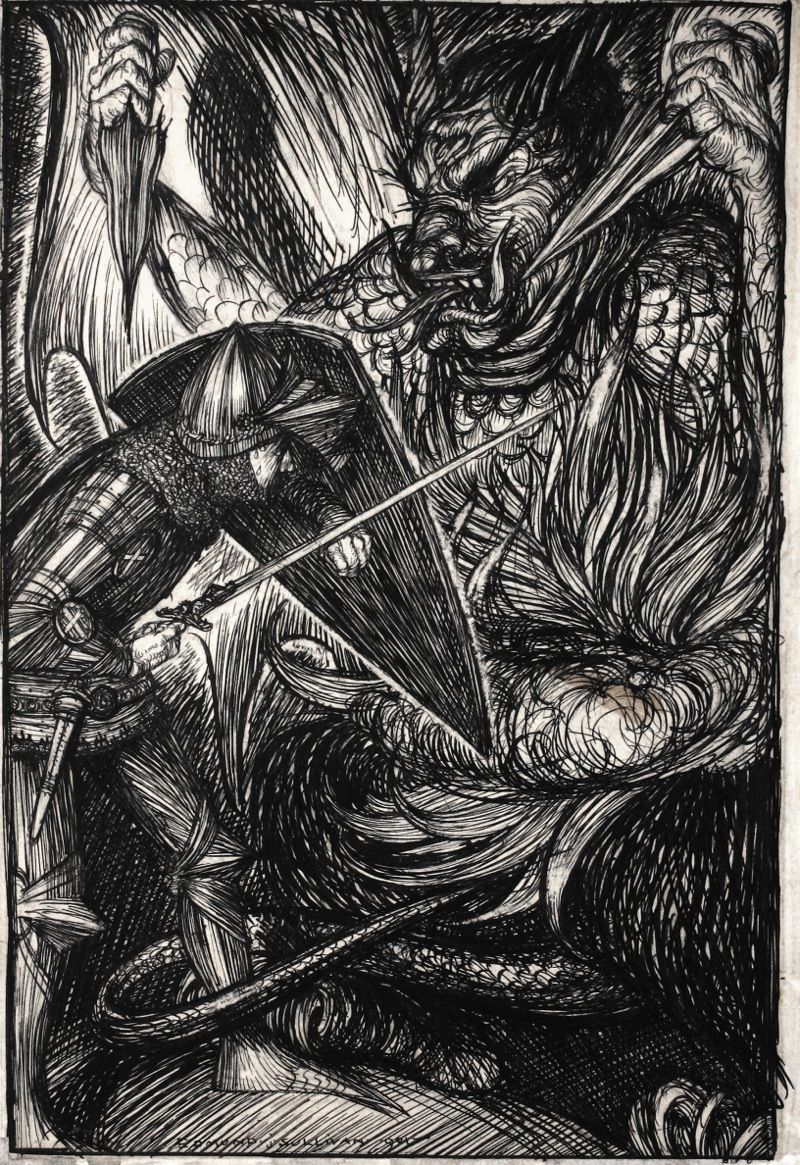
\includegraphics[width=\textwidth]{images/placeholder_image.jpg}}
\vspace*{\fill}
\clearpage

\mainmatter

\chapter*{A Love-Letter}

\begin{center}
    \textit{from the mariner Ulysses}\\
    \textit{to his beloved lady-physician}\poeticmarginnote{ES}
\end{center}

\bigskip

\settowidth{\versewidth}{Like mine can bear and still stay whole.}
\begin{verse}[\versewidth]
    That you're still, in a sense, a virgin,\\*
    Drink like \textit{George Best} and speak like \textit{Charles Spurgeon}\\
    Are all the grounds for love a soul\\
    Like mine can bear and still stay whole.\\
    Two wretched things have kept me up of late,\\
    Which bruise an honest seaman's trust in fate:\\
    The young \& winsome aged, or killed by traffic;\\*
    A girl like you beguiled by all things sapphic.\\!

    Alas, I'm more like \textit{Mars} than \textit{Venus},\\*
    But does that have to come between us?\\
    I'm told I'm gifted with my fingers,\\
    And, though I've not tried cunnalingus,\\
    You're welcome to compare my lips\\
    To any temptress' tastebud-tips,\\
    And summon cries of joy, not laughter.\\*
    (I'd even like to cuddle after.)\\!

    Although I cannot make my chest hair\\*
    Go, and put a plump round breast there,\\
    Nor bid my size 10 feet farewell,\\
    The same goes for my love as well.\\
    Salt-laced hearts do not find in rejection\\
    Grounds for loss of ardour or dejection.\\
    Time will only say, I told you so;\poeticmarginnote{Auden}\\
    And yet it suits me more than you know\\*
    To play \textit{Tiresias} to your virago.
\end{verse}


\chapter*{Another Letter}

\begin{center}
    \textit{from the king Ptolemy Physcon}\\
    \textit{to his beloved daughter-wife}\poeticmarginnote{TM}
\end{center}

\bigskip

\settowidth{\versewidth}{That you are, in your way, one of my daughters}
\begin{verse}[\versewidth]
    That you are, in your way, one of my daughters\blfootnote{The Greek pharoah Ptolemy VIII (he was nicknamed Physcon or ``the Sausage'' on account of his obesity) was surely one of the most wicked and repulsive men ever to have lived. He seduced and later married a girl who had the dubious distinction of being both his niece and his stepdaughter, and later murdered his own son and sent the corpse, piece by piece, to the boy's mother, who was also another of his wives and the mother of the aforementioned niece-stepdaughter-wife. Yet the poet finds something compelling, and, indeed, quite human in this supremely cruel and lustful individual.}\blfootnote{Quetzalcoatl was an Aztec deity who appeared at various times as a rattlesnake, a crow, the planet Venus and a duck.}\\*
    \vin Means that I can forgive you your prattle.\\
    You've a rosebud like music over the waters\poeticmarginnote{Byron}\\
    \vin And more shapes than \textit{Quetzalcoatl}.\\
    \vin \vin \textit{Satan} called, the Devil sent me:\\
    \vin \vin \vin A horse is led\\
    \vin \vin \vin But never made to dip his head:\\*
    \vin \vin When the cat's away the mice do plenty.\\!

    It's no good this outliving \textit{Buddy Holly},\\*
    \vin Growing bald of brow \& round of gut;\\
    No more trips to \textsc{Wakefield} on a jolly\\
    \vin With \sfrac{$1$}{$2$} a lb of coke \& some old slut,\\
    \vin \vin No more younger sisters' teenage friends.\\
    \vin \vin \vin But in your eyes\\
    \vin \vin \vin I see where resurrection lies,\\*
    \vin \vin And how it comes to pass and where it ends.\\!

    There's time enough to consider eternity.\\*
    \vin Put hell on the back burner; heaven can wait.\\
    The love of God and my children's paternity\\
    \vin Are truths too dearly-held to abrogate.\\
    \vin \vin For now, forever, my appetite\\
    \vin \vin \vin Is fixed on thighs,\\
    \vin \vin \vin Waists, fingers, heartbeats, cheeks \& eyes,\\*
    \vin \vin Those lips, both wrapped in cloth and in plain\\*
    \vin \vin \vin \vin sight.
\end{verse}


\chapter*{The Orgy at Earls Crescent}

\begin{center}
{\it also by Ptolemy Physcon}
\end{center}

\bigskip
\bigskip

\settowidth{\versewidth}{The orgy at \textsc{Earls Crescent}}
\begin{verse}[\versewidth]
The orgy at \textsc{Earls Crescent}\\*
\vin Was not as I had hoped,\\
Nor making love as pleasant\\*
\vin As when we first eloped.\\!

\textit{Rosie} \& her cider\poeticmarginnote{Laurie Lee}\\*
\vin Once went straight to my head,\\
But now her quim's much wider\\*
\vin And \textit{Peaches Geldof}'s dead.\\!

The threesome with your sister\\*
\vin Was not so sweet a sin\\
As drunken late-night Twister\\*
\vin On the school trip to \textsc{King's Lynn}.
\end{verse}


\chapter*{Epithalamium}

\settowidth{\versewidth}{In the wilderness of this world, which no man understands,}
\begin{verse}[\versewidth]
\vin It's not that she reminds him of his mother\poeticmarginnote{ES}\\*
\vin \vin (Though since when could \textit{Jocasta}'s comeuppance\\
\vin \vin Ever dissuade him from off-limits tuppence?)\\
\vin But the way they are with one another:\\
In the wilderness of this world, which no man understands,\poeticmarginnote{Bunyan}\\*
She held a little light for him between her hands.
\end{verse}


\chapter*{An Encomium}

\begin{center}
\textit{in praise of The Rev}\\
\textit{Chris Betson, the beloved Vicar}\\
\textit{of St Mary's Tickhill}
\end{center}

\bigskip

\settowidth{\versewidth}{His preaching brings to mind those fearsome creatures,}
\begin{verse}[\versewidth]
\textsc{Rome} had her Caesars; Brandenburg, \textit{Old Fritz};\blfootnote{Friedrich II, King of Prussia and Elector of Brandenburg (known to we English as ``Frederick the Great'') was nicknamed ``Der Alte Fritz'' by his people, i.e. Old Fritz.}\\*
\vin Now \textsc{Tickhill Church} can claim as squire \& master\\
The crimson-haired clergyman we love to bits,\\
\vin Our shield \& broadsword, friend and pastor;\\
\vin And should some peril loom, or grave disaster,\\
The parish wardens need no goads nor whips;\\*
He's all over it like a fat girl on chips.\\!

His preaching brings to mind those fearsome creatures,\\*
\vin \textit{Jan Sobieski} and the Prussian Duke.\blfootnote{Jan III, King of Poland and Grand Duke of Lithuania was named ``Saviour of Christendom'' by the Pope for lifting the siege of Vienna. Albert, Duke of Prussia was the first Protestant head of state.}\\
His writings rank beside the best-loved teachers':\\
\vin \textit{Paul of Tarsus} who -- now please don't puke --\\
\vin Might have had a soft spot for St \textit{Luke},\\
\textit{John Divine} to whose strange works men soften\\*
Once they're told he snorted coke quite often.\\!

Should your parish lack a priest or vicar\\*
\vin And ours go southward in a puff of smoke,\\
I'd recommend you fill the absence quicker\\
\vin Than a scot spends coin or gets a joke.\\
\vin With whom? The ginger \textit{Spurgeon}, God's top bloke:\\
Better than bovril, sturdier than a stetson,\\*
The incomparable Rev \textit{Chris Betson}.
\end{verse}


\chapter*{Vlissingen}

\settowidth{\versewidth}{It was in an old dutch seaport}
\begin{verse}[\versewidth]
It was in an old dutch seaport,\\*
\vin Pocked with dieso and caul,\\
And five loaves \& two fishes\\*
\vin One side of a warehouse wall.\\!

In late september\\*
\vin And summer going,\\
The waves past the breakwater\\*
\vin To-ing \& fro-ing.\\!

The railings rusted,\\*
\vin Weathervanes weathered away.\\
O my love, my fair one,\poeticmarginnote{ER}\\*
\vin I wish I could stay.
\end{verse}


\chapter*{Operation TELIC}

\settowidth{\versewidth}{I wake, earlier than I would like, while the day}
\begin{verse}[\versewidth]
    I\blfootnote{Operation TELIC was the United Kingdom's contribution to the invasion of Iraq in March 2003. The operation was planned over the preceding Christmas, so that the planners joked bitterly that TELIC stood for ``Tell Everyone Leave Is Cancelled''. The poet imagines himself as one of the more lugubrious of said planners.} wake, earlier than I would like, while the day\\*
    Still lies in darkness -- this dark december,\\
    This snowless, christmasless mid-winter.\\
    I work down at the base: purchasing, planning --\\
    Tidal atlases, spreadsheets \& tables\\
    Of figures -- declarations \& forms\\
    To be filled in, signatures gleaned -- meetings\\
    Sat through \& stared through \& endured. Then\\
    I drive back down the same slick sodium-lit roads\\
    Towards a house unheated \& unknown.\\
    I drive \& drive but cannot help my dreaming:\\
    Those febrile bodies, precious as us to themselves,\\
    Cities \& villages, 40 million souls. But death\\
    Plants his boot-heels in the footsteps of \textit{Abraham}.\\*
    Death tightens his cowl in the shadow of the ziggurats.\\!

    The same stars are burning overhead\\*
    As \textit{Algazel} plotted in the House of Wisdom,\\
    The selfsame lustrous moon -- although\\
    Death sips his wine from skulls of Al Anfal.\\
    Death wipes his swords in the waters of the \textsc{Tigris}.\\
    The axeman stands at the root of the tree.\\
    Blood to be shed cries out from the ground -- and yet\\
    The skies are silent. Time alone will tell\\*
    Who was right and if it was all worth it.
\end{verse}


\chapter*{An Elegy for J R H Stoke}

\begin{center}
\textit{whose ashes were buried}\\
\textit{on Blacklyne Common}
\end{center}

\bigskip

\begin{center}
\textsc{i}
\end{center}

\settowidth{\versewidth}{It felt like it was still summer. We drank}
\begin{verse}[\versewidth]
When I came to see you last october\\*
It felt like it was still summer. We drank\\
Warm guinness in a pub in \textsc{Holly Bank}.\\
You talked about growing old, the {\hoskeroe Advocate},\\
That year's lachrymose undergraduate,\\*
How you'd gentle \& disrobe her.\\!
\end{verse}

\bigskip

\begin{center}
\textsc{ii}
\end{center}

\settowidth{\versewidth}{It felt like it was still summer. We drank}
\begin{verse}[\versewidth]
Later, we finished our drinks and \textit{Bernie}\\*
Drove us back into town. The rosy streetlights\\
Recalled lost prep school days and winter nights\\
Beneath a restless wood, and all the while\\
Your lapis blue big eyes \& tender smile,\\*
Like some \sfrac{$1$}{$2$} sweet lines of \textit{Ivor Gurney}.\\!
\end{verse}

\bigskip

\begin{center}
\textsc{the epitaph}
\end{center}

\settowidth{\versewidth}{It felt like it was still summer. We drank}
\begin{verse}[\versewidth]
\it Earth, receive these ashes for safekeeping,\\*
And him, like the \textsc{Black Lyne} flowing:\\
Always running downstream but never going,\\
With strakes \& siltbanks \& silver overlaid,\\
The handsomest of all beds ever made\\*
For man or beast, but not for sleeping.
\end{verse}


\chapter*{Lucifer in Starlight}

\settowidth{\versewidth}{Mapped out both hell's hinterland \& borough,}
\begin{verse}[\versewidth]
I've drank with darkness, shaken hands with sorrow,\\*
Mapped out both hell's hinterland \& borough,\\
Eavesdropped on anguish, glimpsed through grief's gilt lock:\\*
Only the pain itself is too bright to look.
\end{verse}




\bigskip
\bigskip
\begin{center}
\textsc{End of the Second Book}
\end{center}

\end{document}
